\documentclass{article}
\usepackage{tikz}

\begin{document}

\begin{figure}[h]
    \centering
    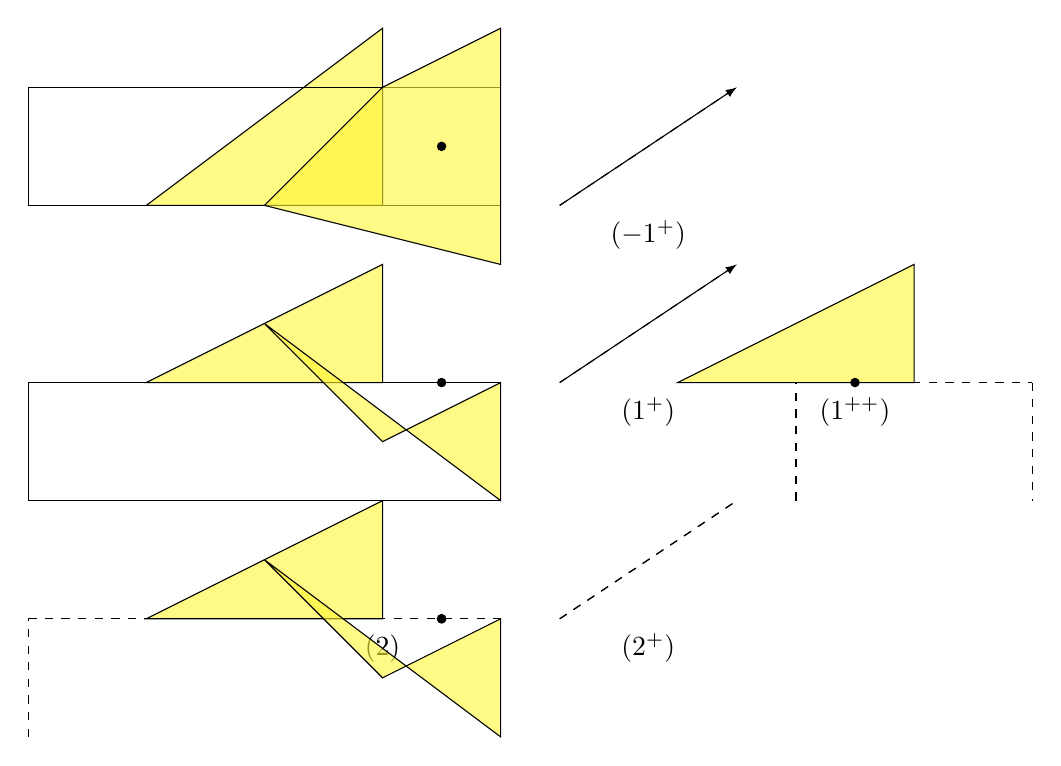
\begin{tikzpicture}[scale=0.75]

        % Region -1*
        \draw[dashed] (-4,-1) -- (4,-1);
        \draw[fill=yellow!80!white, fill opacity=0.6] (-2,-1)--(2,-1) -- (2,2) --cycle;
        \draw (-4,-1) rectangle (4,1);
        
        % Region -1+
        \draw[-latex] (5,-1) -- (8,1);
        \draw[dashed] (5,-1) -- (8,1);
        \node at (6.5,-1.5) {$( -1^{+} )$};
        
        \draw[fill=yellow!80!white, fill opacity=0.6] (4,-2)--(4,2) -- (2,1) -- (0,-1) -- cycle;
        \draw[fill=black] (3,0) circle (2pt);
        
        % Region 1*
        \draw[dashed] (-4,-4) -- (4,-4);
        \draw[dashed] (-4,-6) -- (-4,-4);
        \draw[dashed] (4,-4) -- (4,-6);
        \draw[fill=yellow!80!white, fill opacity=0.6] (-2,-4)--(2,-4) -- (2,-2) --cycle;
        \draw (-4,-6) rectangle (4,-4);
        
        % Region 1+
        \draw[-latex] (5,-4) -- (8,-2);
        \draw[dashed] (5,-4) -- (8,-2);
        \node at (6.5,-4.5) {$( 1^{+} )$};
        
        \draw[fill=yellow!80!white, fill opacity=0.6] (4,-6)--(4,-4) -- (2,-5) -- (0,-3) -- cycle;
        \draw[fill=black] (3,-4) circle (2pt);
        
        % Region 1++
        \draw[dashed] (9,-4) -- (13,-4);
        \draw[dashed] (9,-6) -- (9,-4);
        \draw[dashed] (13,-4) -- (13,-6);
        \draw[fill=yellow!80!white, fill opacity=0.6] (7,-4)--(11,-4) -- (11,-2) --cycle;
        \node at (10,-4.5) {$( 1^{++} )$};
        
        \draw[fill=black] (10,-4) circle (2pt);
        
        % Region 2*
        \draw[dashed] (-4,-8) -- (4,-8);
        \draw[dashed] (-4,-10) -- (-4,-8);
        \draw[dashed] (4,-8) -- (4,-10);
        \draw[fill=yellow!80!white, fill opacity=0.6] (-2,-8)--(2,-8) -- (2,-6) --cycle;
        \draw[fill=black] (3,-8) circle (2pt);
        
        \node at (2,-8.5) {$( 2 )$};
        
        % Region 2+
        \draw[dashed] (5,-8) -- (8,-6);
        \draw[dashed] (5,-8) -- (8,-6);
        \node at (6.5,-8.5) {$( 2^{+} )$};
        
        \draw[fill=yellow!80!white, fill opacity=0.6] (4,-10)--(4,-8) -- (2,-9) -- (0,-7) -- cycle;
        \draw[fill=black] (3,-8) circle (2pt);
        
    \end{tikzpicture}
    
    \caption{Region $M^{\rm I}(i)$ of possible $t$, for $i=\bullet$ in regions labeled by $-1^*$, $1^*$, $2^*$.}
    \label{fig:regions}
\end{figure}

\end{document}